\def\year{2019}\relax
%File: formatting-instruction.tex
\documentclass[letterpaper]{article} %DO NOT CHANGE THIS

\usepackage{aaai19}  %Required
\usepackage{times}  %Required
\usepackage{helvet}  %Required
\usepackage{courier}  %Required
\usepackage{url}  %Required
\usepackage{graphicx}  %Required
\frenchspacing  %Required
\setlength{\pdfpagewidth}{8.5in}  %Required
\setlength{\pdfpageheight}{11in}  %Required
% packages
\usepackage{booktabs} % For formal tables
\usepackage{algorithm}
\usepackage{algpseudocode}
\usepackage{amsmath,amssymb,amsfonts}
\usepackage{graphicx}
\usepackage{xcolor}
\usepackage{todonotes}
\usepackage{xspace}
\usepackage{multirow}
\usepackage{bm}
\usepackage{paralist}
\usepackage{makecell}
\usepackage{xspace}
\usepackage{subcaption}
\usepackage{float}
\usepackage{catchfilebetweentags}
\usepackage[inline]{enumitem}
\usepackage{changepage}
\usepackage{natbib}
\usepackage{xcolor,colortbl, soul, color}
%\usepackage[many]{tcolorbox}
%\usepackage{tikz}
\usepackage{listings}
\DeclareCaptionType[fileext=ext]{program}
\setitemize{noitemsep,topsep=0pt,parsep=0pt,partopsep=0pt}
\newcommand{\algoname}[1]{\textnormal{\textsc{#1}}}
\definecolor{LightCyan}{rgb}{0.88,1,1}
\definecolor{Gray}{gray}{0.9}
\newcolumntype{g}{>{\columncolor{Gray}}c}
\newcolumntype{v}{>{\columncolor{LightCyan}}c}
%PDF Info Is Required:
  \pdfinfo{
/Title (6.867 Project Report - Predicting types in TypeScript using Graph Neural Nets)
/Author (Shashank Srikant)}
\setcounter{secnumdepth}{2}

\makeatletter
    \renewcommand{\copyright@on}{F}
\makeatother

\begin{document}
% env
\newcommand{\loadFig}[1]{
	\ExecuteMetaData[figures.tex]{#1}
}
\newcommand{\loadTbl}[1]{
	\ExecuteMetaData[tables.tex]{#1}
}
\newcommand{\loadCode}[1]{
	\ExecuteMetaData[codes.tex]{#1}
}
\floatstyle{plain}
\newfloat{Grammar}{tb}{cog}
\newcommand{\progname}[1]{{\small\texttt{#1}}\xspace}
\newcommand{\smallname}[1]{{\small{#1}}\xspace}
\newcommand{\prognamenox}[1]{{\small\texttt{#1}}}

\newcommand{\rs}{\textit{Representation stack}\xspace}
\newcommand{\use}{\textit{use}\xspace}
\newcommand{\define}{\textit{define}\xspace}
\newcommand{\usedef}{\texttt{Use \& Define}\xspace}
\newcommand{\used}{\textit{used}\xspace}
\newcommand{\defined}{\textit{defined}\xspace}

\newcommand{\My}{\textsf{M}\xspace}
\newcommand{\Oy}{\textsf{O}\xspace}

\newcommand{\Tok}{\progname{T}}
\newcommand{\TokNoOp}{\progname{Node}}

\newcommand{\UU}{\progname{U}}
\newcommand{\UUT}{\progname{U+T}}
\newcommand{\UUO}{\progname{U+Op}}

\newcommand{\UD}{\progname{UD}}
\newcommand{\UDT}{\progname{UD+T}}
\newcommand{\UDO}{\progname{UD+Op}}

\newcommand{\DD}{\progname{D}}
\newcommand{\DDT}{\progname{D+T}}
\newcommand{\DDO}{\progname{D+Op}}

\newcommand{\DU}{\progname{DU}}
\newcommand{\DUT}{\progname{DU+T}}
\newcommand{\DUO}{\progname{DU+Op}}

\newcommand{\UDU}{\progname{U+D+UD}}
\newcommand{\UDUT}{\progname{U+D+UD+T}}

\newcommand{\es}{\progname{ExceptSt}}
\newcommand{\of}{\progname{IntOv}}
\newcommand{\uf}{\progname{IntUn}}
\newcommand{\ec}{\progname{ExtCall}}
\newcommand{\mc}{\progname{MultCalls}}
\newcommand{\sch}{\progname{StateChange}}
\newcommand{\tod}{\progname{TOD}}

\newcommand{\esbof}{\bf{\progname{ExceptSt}}}
\newcommand{\ofbof}{\bf{\progname{IntOv}}}
\newcommand{\ufbof}{\bf{\progname{IntUn}}}
\newcommand{\ecbof}{\bf{\progname{ExtCall}}}
\newcommand{\mcbof}{\bf{\progname{MultCalls}}}
\newcommand{\schbof}{\bf{\progname{StateChange}}}
\newcommand{\todbof}{\bf{\progname{TOD}}}
\newcommand{\bof[1]}{\textbf{#1}}

\newcommand{\calv}{$v$\xspace}
\newcommand{\calG}{$\mathcal{G}$\xspace}
\newcommand{\calGp}{$\mathcal{G'}$\xspace}
\newcommand{\calP}{$\mathcal{P}$\xspace}
\newcommand{\calS}{$\mathcal{S}$\xspace}
\newcommand{\calT}{$\mathcal{T}$\xspace}

\newcommand{\etc}{\textit{etc}.\xspace}
\newcommand{\ie}{\textit{i.e.}\xspace}
\newcommand{\eg}{\textit{e.g.}\xspace}
\newcommand{\ra}{$\rightarrow$}

\newcommand{\TODO}[1]{\textcolor{blue}{TODO: #1}}
\newcommand{\FIX}[1]{\textcolor{red}{CHECK: #1}}
\newcommand{\COMMENT}[1]{\textcolor{red}{COMMENT: #1}}

\newcommand{\rarro}[1][3pt]{\mathrel{%
		\hbox{\rule[\dimexpr\fontdimen22\textfont2-.2pt\relax]{#1}{.4pt}}%
		\mkern-4mu\hbox{\usefont{U}{lasy}{m}{n}\symbol{41}}}}

\newcommand{\rarr}{$\rarro$}

\newcommand{\scl}{0.5}
\newcommand{\wdth}{0.28}

\newcommand{\colorul}[2]{\setulcolor{#1}\ul{#2}}
\definecolor{ogreen}{rgb}{0.0, 0.8, 0.6}
\newcommand{\bx}[2]{
 \begin{tikzpicture}
 \node[draw,dashed,fill={#1!10}] {{#2}};
 \end{tikzpicture}
}

\setul{0.2ex}{0.4ex}
\makeatletter
\def\BState{\State\hskip-\ALG@thistlm}
\makeatother
\title{\Large{Modeling Computer Programs: A Case Study in Predicting Variable Types via Graph Neural Nets}
	\\~\\
	\small{Project URL: \url{https://github.com/shashank-srikant/6.867_term_project/}}
}

\author{Alex Renda, Katie Lewis, Shashank Srikant
\\
CSAIL, MIT
\\
\{renda, kmlewis, shash\}@mit.edu
}
\maketitle

\begin{abstract}
	We explore the problem of modeling computer programs to infer their properties.
We argue that programs can be modeled as Markov Random Fields, where the latent random variables in the graph represent the properties of interest.
We approximate inference over such a graphical model via graph neural networks (GNN), a neural network architecture which captures graph-like structural information.
As a case study, we work on the problem of inferring variable types in JavaScript programs.
We show that modeling this task using GNNs provides a 10-15\% improvement in accuracy of type prediction when compared to a bi-directional RNN baseline.
Via ablation studies, we also investigate the benefits of various modeling assumptions we make in our GNN construction.
\end{abstract}
\section{Introduction}
\label{sec:introduction}
Inferring properties of computer programs is a task central to the programming languages (PL) community. Although important questions like whether a program shall terminate, or finding a test case which shall crash a program are undecidable, the program analysis community, over the last few decades, has designed algorithms and techniques which solve such undecidable problems to a good approximation, and to an extent where such solutions have been shipped to real-time, commercial products.

One such property of interest is ascertaining types of variables used in programs. Static, strongly-typed languages provide considerable guarantees at compile-time, enabling programmers to write bug-free, well understandable code. Although the advantages of this paradigm have been well understood by the programming community, there exist many popular languages such as Python, Ruby, and Javascript which do not enforce static typing. These languages prevent typing errors at run-time, and do little type-checking at compile-time. This approach of exclusive dynamic typing is referred to as \textit{duck-typing}. Despite the various pros and cons of duck-typing, it is widely adopted and is used extensively in production systems. This warrants some form of retrospective ability which can provide, at compile time, type-information with an acceptable degree of accuracy.

One approach to having such retrospective type-checking on a language which does not inherently support static type checking is having programmers provide partial information on types of variables used in their programs. This enables established type-inference algorithms to determine types of various variables used in a program, and is bound by the amount of annotation which a user provides. Another approach, which is the subject of this work, is to infer types statistically. The problem of inferring types can be cast as one in supervised machine learning, wherein from a given corpus of programs with identified types, supervised models can infer types of unseen variables, in unseen programs.

This broader approach has been validated with a modest degree of success in previous work \cite{}. Allamanis et al. modeled the problem as a sequence translation task, and trained bi-directional RNNs to predict types (see Section \ref{sec:relatedwork}). In this work, we ask whether there are inductive biases which are unique to the input space - computer programs, and whether they can be exploited in such a prediction task. We motivate this problem as an inference task over a probabilistic graphical model, and approximate it using a graph-based neural networks. We show that such a modeling approach does better than modeling it as a sequence prediction task.


%%% Local Variables:
%%% TeX-master: "main"
%%% End:
\section{Motivation}
\label{sec:motivation}
\subsubsection{.}
background 
\subsubsection{Graph neural networks.} 
some more background
\section{Approach}
\label{sec:approach}

Our approach to the type prediction problem is to apply a GNN to a special graph constructed from each TypeScript program, where the graph encodes much of the information that may be relevant in trying to predict a given variable's type.

\subsection{Dataset}
\label{sec:dataset}
We borrowed from the dataset which the DeepTyper project worked on \cite{hellendoorn2018deep}. 1000 top starred open-source projects on Github that predominantly consisted of TypeScript codes were parsed. Each project was parsed with the TypeScript compiler \textsc{tsc}, which infers type information (possibly any) for all occurrences of each identifier. A total of 90 projects, containing 5000 source codes, resulting in 650,000 labels were finally used in our experiments.
For our prediction problem, to avoid the sparsity problems that come with such a large label set, we throw out all labels that are not in the top 20 most common labels, which combined counts for roughly $50\%$ of the total labels in the training dataset.
The CDF of label frequencies can be seen in Figure~\ref{fig:lab-cdf}, showing the long tail of infrequent labels.
To give a better idea of the type labels that we predict, the top 5 most common types in the training set are: \texttt{string}, \texttt{number}, \texttt{boolean}, \texttt{any[]}, and \texttt{string[]}.

\begin{figure}
  \centering
  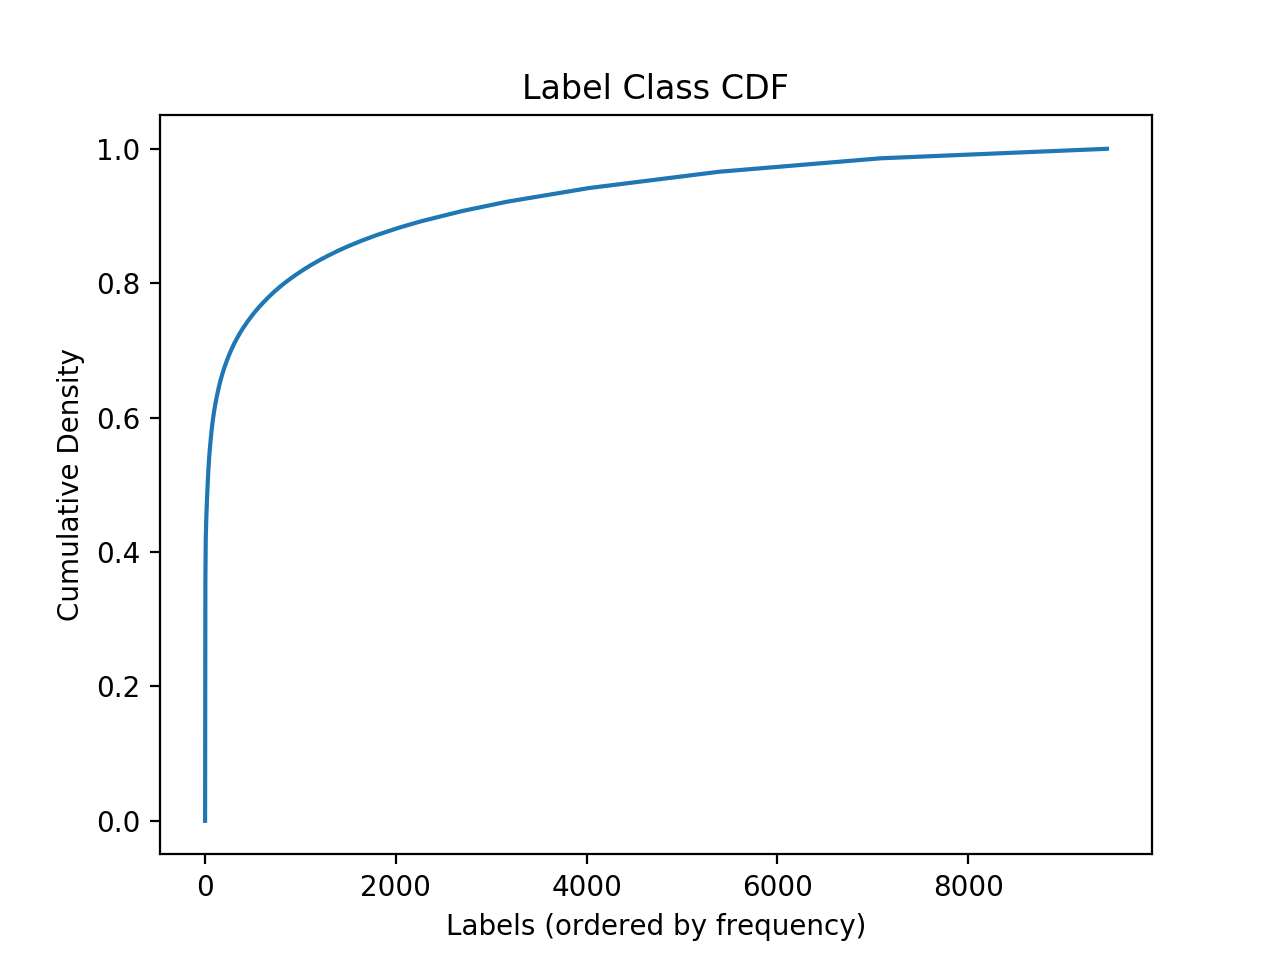
\includegraphics[width=\linewidth]{img/label_cdf}
  \caption{Distribution of label frequencies in training dataset}
  \label{fig:lab-cdf}
\end{figure}

\paragraph{Train-Test split.}

We made sure to do our train/test split on the dataset not based on files, but on projects, since we are primarily interested in how this approach performs on code that it has never seen before.
Files within the same project do tend to have similar, even identical code snippets, so we wanted to rule out any potential false positives from memorizing such sub-graphs.
This is, however, a conservation model of a real world system: a type predictor built into an IDE would have access to other files within the same project that the user has written, and would be able to base predictions on that.
Because of this, we have a separate set of weights for computing the initial node and edge embeddings, so that a model can refine its training on graphs specific to one type of project, while keeping the same node/edge embeddings and predictors, essentially performing a version of the standard NLP-style transfer learning, but for program graphs.

\subsection{Graph construction.}

Because ``graph neural nets'' are such a general framework, the inductive bias for the solution comes primarily from how the input graph is constructed.
Specifically, we must decide on the nodes and edges of our generated graph.
We choose to include the full set of nodes in each program's AST as the nodes in the input graph, using the node's syntactic token type as its embedding.
This allows us to include all potentially relevant structure: we have not only the source level tokens in the source file, but also the abstract structures that those tokens form.

Graph edges are significantly more complicated.
We want to take advantage of all of the important connections that we know about in the program, while also trying to avoid creating as many useless edges as possible, both to help with computation and to induce a stronger prior over the solutions we think might be valid.
Specifically, we take advantage of our knowledge of the important local and nonlocal interactions between various parts of programs, similar to how convolutional networks assume some strong relationship between local pixels~\cite{henaff2015deep}.
There are three specific priors we bake into the edges in our generated graph:

\paragraph{Nodes near a variable in the AST reflect something about that variable's type.}\
\ % need a space after paragraph
\begin{lstlisting}
  let x = y * 2;
\end{lstlisting}
A human trying to infer the type of the variable \texttt{x} in the above code may decide that since the result of multiplying something by a number is almost always a number, \texttt{x} is probably a number.
This corresponds exactly to two types of edges that we include in our generated graph, an \texttt{AstChild} edge from parents to their child nodes in the AST, and an \texttt{AstParent} edge from children to their parent in the AST.

\par\paragraph{Nodes near a variable in the file reflect something about that variable's type.}
\ % need a space after paragraph
\begin{lstlisting}
  let x = 1;
  let y = x;
  ...
  let x = "foo";
\end{lstlisting}
It is clear that both ordering and locality matter in determining the type of \texttt{y}: in the AST, the two statements assigning to \texttt{x} are equidistant and directionally indistinguishable, but the actual \emph{token stream} of file reflects that the first assignment to \texttt{x} precedes the assignment to \texttt{y}, meaning that it may be more likely to affect the type of \texttt{y}, and is also closer, meaning the two statements are more likely to be related.
Because of this, we include two more types of edges in the induced graph, a \texttt{TokenNext} edge from a token to its neighbor in the source file, and a \texttt{TokenPrev} edge which is the reverse.

\paragraph{Nodes that use or define the same variable give information about each other.}
\ % need a space after paragraph
\begin{lstlisting}
  let x = 1;
  ...
  let y = a + (b + (... + x));
\end{lstlisting}
Although the two statements may be arbitrarily nonlocal in both the AST and the source file, they are clearly related, in that \texttt{x}'s type probably influences \texttt{y}'s type.
Because of this, we include one final types of edge, a \texttt{Variable} edge between any of a variable's use and definition.

\paragraph{Example.}
With all of the above nodes and edges included, we generate (a cleaned up version of) the graph shown in Figure~\ref{fig:ast-graph} for the following problem:
\begin{lstlisting}
  let x := 5;
  x = x + 2;
  console.log(x);
\end{lstlisting}

\begin{figure}
  \centering
  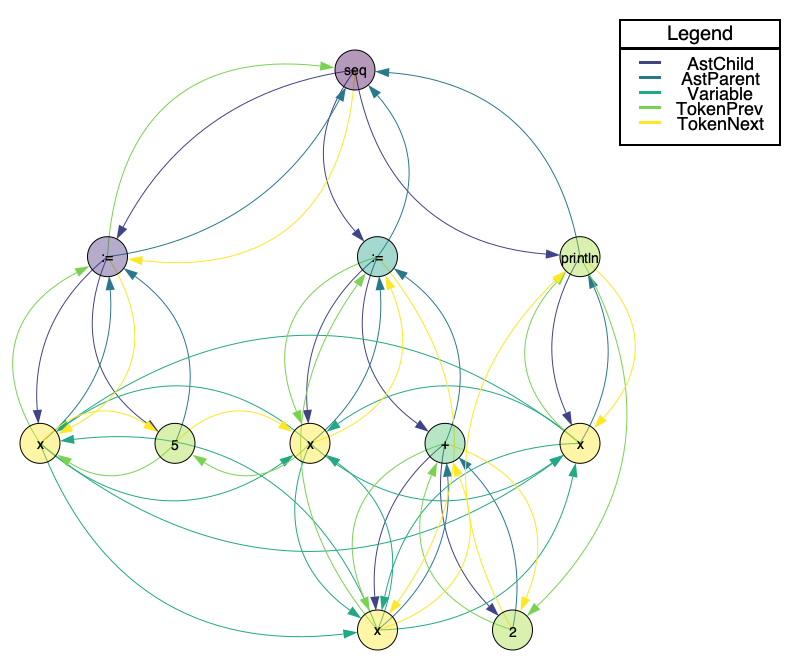
\includegraphics[width=\linewidth]{img/gen_graph}
  \caption{Generated graph for a simple example}
  \label{fig:ast-graph}
\end{figure}

\subsection{Embeddings.}

In the program graph, a node's initial embedding is a one-hot vector encoding its AST type.
Similarly, an edge's embedding is a one-hot vector encoding its edge type.
We keep the top 60 node types, and consolidate the rest into an \textsc{Unk} token, to avoid sparsity on the bottom end of the node type distribution (the distribution of AST node types in our dataset can be seen in Figure~\ref{fig:ast-cdf}; the top 60 node types correspond to $95\%$ of all ndoes).
We do not do the same with edge types, since by construction all edge types are densely populated.

\subsection{Architecture.}

The graph architecture we explore is fairly simple, with minimal observed effects from architecture tuning.
The core of the architecture is the graph neural net, described in Section~\ref{sec:graph-neural-net}.
To use this, we perform some minor pre- and post-processing on the data: we have a one-hidden-unit fully connected layer to transform the one-hot encodings into the initial node and edge embeddings, and after running the graph, we similarly have a one-hidden-unit fully connected layer to transform the final latent state into the predictions.
These two fully connected layers are the parts held constant for the transfer learning approach mentioned above, in Section~\ref{sec:dataset}.

\subsection{Implementation.}

We implemented our type prediction algorithm using using DeepMind's Graph Nets framework~\cite{deepmind2018graph}, along with a significant amount of custom TensorFlow~\cite{google2015tensorflow} to collect metrics and perform experiments.
Our implementation, along with minor extensions to the Graph Nets framework, can be found online\footnote{\url{https://github.com/shashank-srikant/6.867_term_project/blob/master/src/graph_neural_net/nn.py}}.
\section{Experiments}
\label{sec:experiments}
We investigate the following questions in this work, and set up experiments to answer them.

\begin{itemize}[noitemsep,topsep=0pt]
	\item \textbf{E1.} Do GNNs capture well the inductive bias in representing prediction tasks with a graph-like structure?
	\item \textbf{E2.} How does the nature of structural information passed along the edges in a GNN affect its predictability?
	\item \textbf{E3.} How can the number of iterations, a critical hyperparameter which controls message passing in graph networks, be determined automatically, as against the current way of setting them apriori?
\end{itemize}

\subsubsection{Experiment 1. Representation using GNN.}
We investigate whether the inductive bias captured in the structure of graph neural networks help in prediction tasks on graph-like modalities. To determine this, we model the task of predicting types of variables using GNN. To ascertain whether the architecture naturally captures this prediction task, we set up a number of baselines to compare against. We investigated the following models -
\begin{itemize}[noitemsep,topsep=0pt]
	\item \textbf{Our model. GNN.} We model the type inference problem using GNNs. Each node represents a node in the program's AST. We infer the types on those nodes which pertain to a variable. This is the model we compare all other baselines against.
	\item \textbf{Baseline 1. Naive.} We design a naive baseline to compare performance. In this model, we perform a majority vote on the label distribution in our train-set, and use the most frequently occurring label as the type predicted for any unseen variable. This provides a maximum likelihood estimate.
	\item \textbf{Baseline 2. Intermediate.} Increasing the complexity of our baseline models, we evaluate a naive approximation of a graph net. In this model, we construct a logistic regression model over a feature vector involving \textit{counts} of various dependency and node information of a program. Specifically, for each program in the corpus, we enumerate the following counts
	\begin{itemize}[noitemsep,topsep=0pt]
		\item Edges between every \textsc{VariableUse} and \textsc{VariableDefine}, as described in Section \ref{sec:approach}. This forms a \textit{count}-hot vector of all such unique edge-dependencies that appear in the training corpus.
		\item A  \textit{count}-hot encoding of the AST node types that appear in a program.
	\end{itemize}
	We enumerated XX different edge types and YY unique AST nodes in the training set. This resulted in a AAxBB feature matrix, which was used to learn a Logistic Regression model. This baseline captures a \textit{bag-of-dependencies}, without the structural/directional information provided by GNNs.
	\item \textbf{Baseline 3. Aggressive.} We use the bi-directional neural network architecture designed by Allamanis et al \cite{hellendoorn2018deep}. Their architecture does not utilize any of the graphical-properties of a program, and instead rely on signals obtained just by the token information. Their approach is typical of sequence prediction tasks in NLP. Figure \ref{fig:birnn} describes their architecture.
\end{itemize}
this is 
\loadFig{baseline}
\subsubsection{Experiment 2. Edge information - Ablation study.}
To determine whether our graph structure (nodes and edges) was chosen correctly, we performed a set of ablation studies.
Specifically, we ran experiments using the optimally chosen hyperparameters where we entirely deleted each class of edges (AST edges, Token edges, and Variable edges) from the graph, and compared performance to the original.
The results of these studies can be seen in Tables~\ref{tab:results:ast}, \ref{tab:results:variable}, and \ref{tab:results:token}.
These experiments confirm our assumptions, that each of the types of edges we selected help in solving the type inference problem.
We can additionally see the relative benefit of each of the edge types: the syntactic locality induced by the \textsc{Token} edges seems to matter more than the AST edges, which in turn matter more than the \textsc{Variable} edges.
While it is somewhat surprising that the \textsc{Variable} edges are the least important, since type inference is based in part on variable usage, this can be explained in part by the relatively small number of message passing iterations: there is no immediate information gained from a linked variable, only from that linked variable's neighbors, so more iterations would likely be needed to see as much benefit from the \textsc{Variable} edges.

\subsubsection{Experiment 3. Number of iterations.}
A shortcoming in the graph net framework is the issue of determining how many iterations to run.
In theory, because of the universal approximation properties of neural nets, the optimal number of iterations is any number larger than the diameter of the graph, so that each node can make a fully informed decision knowing the entire graph topology.
However, this is not realistic: as shown in Figure~\ref{fig:dataset-graph-stats}, the maximum diameter of any of the graphs is above 200, meaning that we would have to run the graph neural net for an intractable number of iterations to be able to get the ``full'' result.
Instead, we approximate the result by running fewer iterations, theoretically losing out on certain classes of decisions (although further enforcing our inductive bias, since we believe that local nodes should be the primary ones that matter).
It is not immediately clear how we should choose the \textsc{NIter} hyperparameter though: since graph nets give no formal guarantees that the results monotonically improve with the number of iterations, we have to select the number of iterations through some hyperparameter search.
We ran two experiments to try to select the ideal settings: a \emph{Bayesian Optimization} based approach, and what we call an \emph{Iteration Ensemble} approach.

\paragraph{Bayesian Optimization.}
Our first attempt at finding the ideal number of iterations was inspired by standard approaches to hyperparameter search problems, for cases where running experiments can be prohibitively expensive (the memory and time costs of training a model means we can only search through a relatively small number of possible hyperparameters).
In particular we were inspired by \cite{snoek2012practical}, which suggests using a Bayesian Optimization based approach with an underlying Gaussian Process to pick hyperparameters, using the expected improvement metric (expectation of the decrease in the desired metric over the current best known hyperparameter) to explore the hyperparameter space.
The metric we chose to optimize over was the train loss after 3 epochs.
Selecting the best performing number of iterations in this metric gave us confidence that the network had actually made progress in learning significant features of the dataset, while also being sure not to overfit to our validation set.
The results of this experiment can be seen in Figure~\ref{fig:gp-diagram}, which shows the confidence bounds on the number of iterations to use in the range $[0, 10]$, which gave us a satisfactory coverage of the average path length seen in Figure~\ref{fig:dataset-graph-stats}, while still being computationally tractable to train.
After 5 interactions with the Gaussian process, we were confident that $n=1$ iteration gave the best training loss after 3 epochs, although we used $n=2$ in our experiments, since it seemed to do marginally better on the validation set.

We were slightly surprised by the relatively low number of iterations found as ideal by the Bayesian Optimization.
Ultimately, we believe that this is probably an issue with the amount of time that we trained for: since a message passing graph net unfurls to look similar to a RNN, it encounters the same vanishing gradient problem, magnified by the large fanout of each node (Figure~\ref{fig:dataset-graph-stats} shows an average node degree above 5).
Were we to train for significantly longer, we may be able to deal with the smaller gradients and the more complex loss landscape of a larger network, but unfortunately training the larger \textsc{NIter} networks for longer on our machines was computationally infeasible -- we leave this deeper parameter exploration to future work.

\paragraph{Iteration Ensemble.}
Our second attempt at hyperparameter search followed a more optimization based approach.
Rather than trying to pick one specific ideal number of iterations, we ran an ensemble over several choices of iteration counts, using a learned weighting to linearly combine all of their predictions in the last step to produce the final result.
Importantly, we ran this iteration ensemble on \emph{one single graph net}; that is, we combined each of the intermediate predictions of running a single graph neural net.
We took this approach for two reasons: primarily, it was more computationally efficient (running large ensembles of graph nets was not possible on the machines we had access to), but it also enforced one of the inductive biases we hoped to see in a solution: intermediate steps of the graph net message passing algorithm should roughly correspond to finer and finer approximations of the posterior prediction, meaning all steps should be valid (if unrefined) predictions.
We also hoped to see situations where some weights on the upper or lower end would drop away, signifying that we should shift the number of iterations that comprise the ensemble.

Ultimately, this did not work as well as we hoped, and our best results were achieved by just using a single number of iterations learned through the Bayesian Optimization approach.
The linear combination weight vector changed only marginally from its initial value, and the prediction quality was no better than that of using a fixed number of iterations.
We believe this happened for one primary reason: one or two iterations were good enough, as shown by the Bayesian Optimization approach.
Any iterations beyond that did not refine the search, and since we did not penalize their existence through any regularization (only the wrongness of their predictions), they stayed around as unnecessary artifacts that did not get pruned.
\loadFig{gpDiagram}

\section{Results and Discussion}
\label{sec:results}


\begin{table*}
	\begin{minipage}{.5\linewidth}
		\centering
		{\renewcommand{\arraystretch}{1.3}% for the vertical padding
			\begin{tabular}{c|lcc}
				~ & \textbf{Model} & \textbf{P@1} & \textbf{P@5} \\
				\hline
				Our model & \textbf{GNN} & 0.66 & 0.96 \\
				\hline
				~ & \textbf{Na\"ive} & 0.31 & 0.87 \\
				~	 & (Majority vote) & ~ & ~ \\
				\cline{2-4}
				Baselines & \textbf{Intermediate} & 0.44 & 0.93 \\
				~	 & (Dependency counts) & ~ & ~ \\
				\cline{2-4}
				~	 & \textbf{Aggressive} & 0.50 & * \\
				~	 & (Bi-directional RNN) & ~ & ~ \\
			\end{tabular}
		}
		\caption{Results of model comparison against various baselines, ordered by their model complexity. These are results on the test-set, on the top 20 most frequent labels in the train-set. P@1, P@5 correspond to the accuracy of top-1 and top-5 predictions matching the exact label.}
		\label{tab:results:baselines}
	\end{minipage}
	\begin{minipage}{.5\linewidth}
		\centering
		{\renewcommand{\arraystretch}{1.3}% for the vertical padding
			\begin{tabular}{l|cc}
				\textbf{Ablated Model} & \textbf{P@1} & \textbf{P@5} \\
				\hline
				Full GNN model & 0.66 & 0.96 \\
				AST edges removed &  0.55 & 0.93 \\
				Token edges removed & 0.43 & 0.94 \\
				Use-Define edges removed & 0.61 & 0.92 \\
			\end{tabular}
		}
		\caption{Results of our ablation study.}
		\label{tab:results:ablations}
	\end{minipage}
\end{table*}

\subsubsection{Experiment 1.}
The results of this can be seen in Table~\ref{tab:results:baselines}.
The best results we achieved, using the graph neural net with $\textsc{NIter}=2$ and including all AST, \textsc{Variable}, and \textsc{Token} edges had P@1 and P@5 accuracies of 66\% and 96\% respectively.

Regarding baselines, we see that the \textit{intermediate} baseline performs as expected.
It predicts \textit{number} and \textit{string} types well, and fails at predicting any other type accurately.
Analyzing the model's selected features reveals node types like $+$ are highly weighted, which correspond to operations specific to \textit{number}s and \textit{string}s.
We leave a detailed analysis of these learned features to future work.

The \textit{aggressive} bi-directional RNN baseline, which was the best model trained by Allamanis \textit{et al.}~\cite{hellendoorn2018deep}, performs in the ballpark reported in their work (slightly worse than~\cite{hellendoorn2018deep}, where the variance is explained by the smaller size of our dataset).
It has a P@1 accuracy of 50.6\%, 16\% lower than the GNN's performance.

These results confirm that the graph neural net framework, along with the assumptions we made about the graph structure, work well to model the problem: our solution roughly halves the error rate from random guessing, and significantly outperforms all other baselines.

\paragraph{GNN model diagnosis.}
We also include a sampling of the false positive and negative rates on the test set in Table~\ref{tab:test-fps}.
It shows only two significant outliers, the number of false predictions on the \texttt{string} type and the number of missed predictions of the \texttt{number} type.
Given that some of the most common operators on numbers and strings are syntactically identical in TypeScript ($+$ adds numbers and concatenates strings), it is unsurprising that numbers would get interpreted as strings, especially considering that the MLE guess when the two are syntactically indistinguishable would be \texttt{string}; this intuition has been confirmed by checking that the majority of missed \texttt{number} predictions are predicted as \texttt{string}s.

\subsubsection{Experiment 2.}
The results of the ablation studies can be seen in Table~\ref{tab:results:ablations}.
These experiments confirm our assumptions, that each of the types of edges we selected help in solving the type inference problem.
We can additionally see the relative benefit of each of the edge types: the syntactic locality induced by the \textsc{Token} edges seems to matter more than the AST edges, which in turn matter more than the \textsc{Variable} edges.
While it is somewhat surprising that the \textsc{Variable} edges are the least important, since type inference is based in part on variable usage, this can be explained in part by the relatively small number of message passing iterations: there is no immediate information gained from a linked variable, only from that linked variable's neighbors, so more iterations would likely be needed to see as much benefit from the \textsc{Variable} edges.

\begin{table}
  \centering
  {\renewcommand{\arraystretch}{1.3}% for the vertical padding
  \begin{tabular}{lrrr}
    \textbf{Label} & \textbf{\#Correct} & \textbf{\#Missed} & \textbf{\#FP} \\
    \hline
    \texttt{string} & 6374 & 1021 & 4216 \\
    \texttt{number} & 5501 & 4006 & 881 \\
    \texttt{boolean} & 1610 & 850 & 1089 \\
    \texttt{any[]} & 367 & 240 & 226 \\
    \texttt{string[]} & 130 & 321 & 141 \\
    \texttt{() => void} & 606 & 279 & 190 \\
    \texttt{A}  & 0 & 0 & 301 \\
    \texttt{undefined} & 37 & 58 & 179 \\
    \texttt{() => string} & 91 & 112 & 111
  \end{tabular}
   }
  \caption{Top 10 test labels (23551 total predictions)}\label{tab:test-fps}
\end{table}

\subsubsection{Experiment 3.}
\textbf{Bayesian Optimization.}
The metric we chose to optimize over was the train loss after 3 epochs.
Selecting the best performing number of iterations with this particular metric gave us confidence that the network had actually made progress in learning significant features of the dataset, while also being sure not to overfit to our validation set.
Partial results of this experiment can be seen in Figure~\ref{fig:gp-diagram}, which shows the confidence bounds on the number of iterations to use in the range $[0, 10]$.
These bounds gave us a satisfactory coverage of enough message passing to propagate through the average path in the graph (c.f.~Figure~\ref{fig:dataset-graph-stats}), while still being computationally tractable to train.
After 5 interactions with the Gaussian process, we were confident that $n=1$ iteration gave the best training loss after 3 epochs, although we used $n=2$ in our experiments, since it seemed to do marginally better on the validation set.

We were slightly surprised by the relatively low number of iterations found as ideal by the Bayesian Optimization.
Ultimately, we believe that this is probably an issue with the amount of time that we trained for: since a message passing graph net unfurls to look similar to a RNN, it encounters the same vanishing gradient problem, magnified by the large fanout of each node (Figure~\ref{fig:dataset-graph-stats} shows an average node degree above 5).
Were we to train for significantly longer, we may be able to deal with the smaller gradients and the more complex loss landscape of a larger network, but unfortunately training the larger \textsc{NIter} networks for longer on our machines was computationally infeasible -- we leave this deeper parameter exploration to future work.
\loadFig{gpDiagram}

\paragraph{Iteration Ensemble.}
Ultimately, this experiment did not work as well as we hoped, and our best results were achieved by just using a single number of iterations learned through the Bayesian Optimization approach.
The linear combination weight vector changed only marginally from its initial value, and the prediction quality was no better than that of using a fixed number of iterations.
We believe this happened for one primary reason: one or two iterations were good enough, as shown by the Bayesian Optimization approach.
Any iterations beyond that did not refine the search, and since we did not penalize their existence through any regularization (only the wrongness of their predictions), they stayed around as unnecessary artifacts that did not get pruned.

%\section{Related Work}
\label{sec:related_work}
Recent work have focused on . 
\section{Conclusion}
\label{sec:conclusions}

In this work, we investigate modeling computer programs using graph neural networks. Our results demonstrate that for learning tasks on graph-based structures, the inductive bias introduced by GNNs offers a significant benefit over other modeling choices. For the specific task of type prediction, we show that GNNs perform better than state of the art modeling choices like bi-directional RNNs. We also confirm through experiments the effect the right choice of edge information has on the learning task. We believe a larger research question on formalizing GNNs through the lens of probabilistic graphical modes is wide open.  

\section{Task split-up}
\begin{itemize}[]
	\item \textbf{Alex.}
	\item \textbf{Katie.}
	\item \textbf{Shashank.}
\end{itemize}



\medskip
\bibliographystyle{unsrt}
\bibliography{main}

\end{document}


%%% Local Variables:
%%% TeX-master: "main"
%%% End: